\chapter{Конструкторский раздел}
\label{cha:design}
В этом разделе будут рассмотрены требования к программе и схемы для реализации алгоритмов, математические расчёты.
Программа должна предоставлять возможность:
\begin{itemize}
	\item загружать модель мышц;
	\item вращать и перемещать загруженную модель;
	\item визуализировать мышечные сокращения;
	\item задавать степень сокращения;
	\item добавлять и перемещать источники освещения.
\end{itemize}

\section{Общий алгоритм работы программы}
\label{sec:general}
На рисунках \ref{fig:01a-0} и \ref{fig:02a0} приведены IDEF0 диаграммы, представляющие организацию работы программы.
\begin{figure}[H]
	\centering
	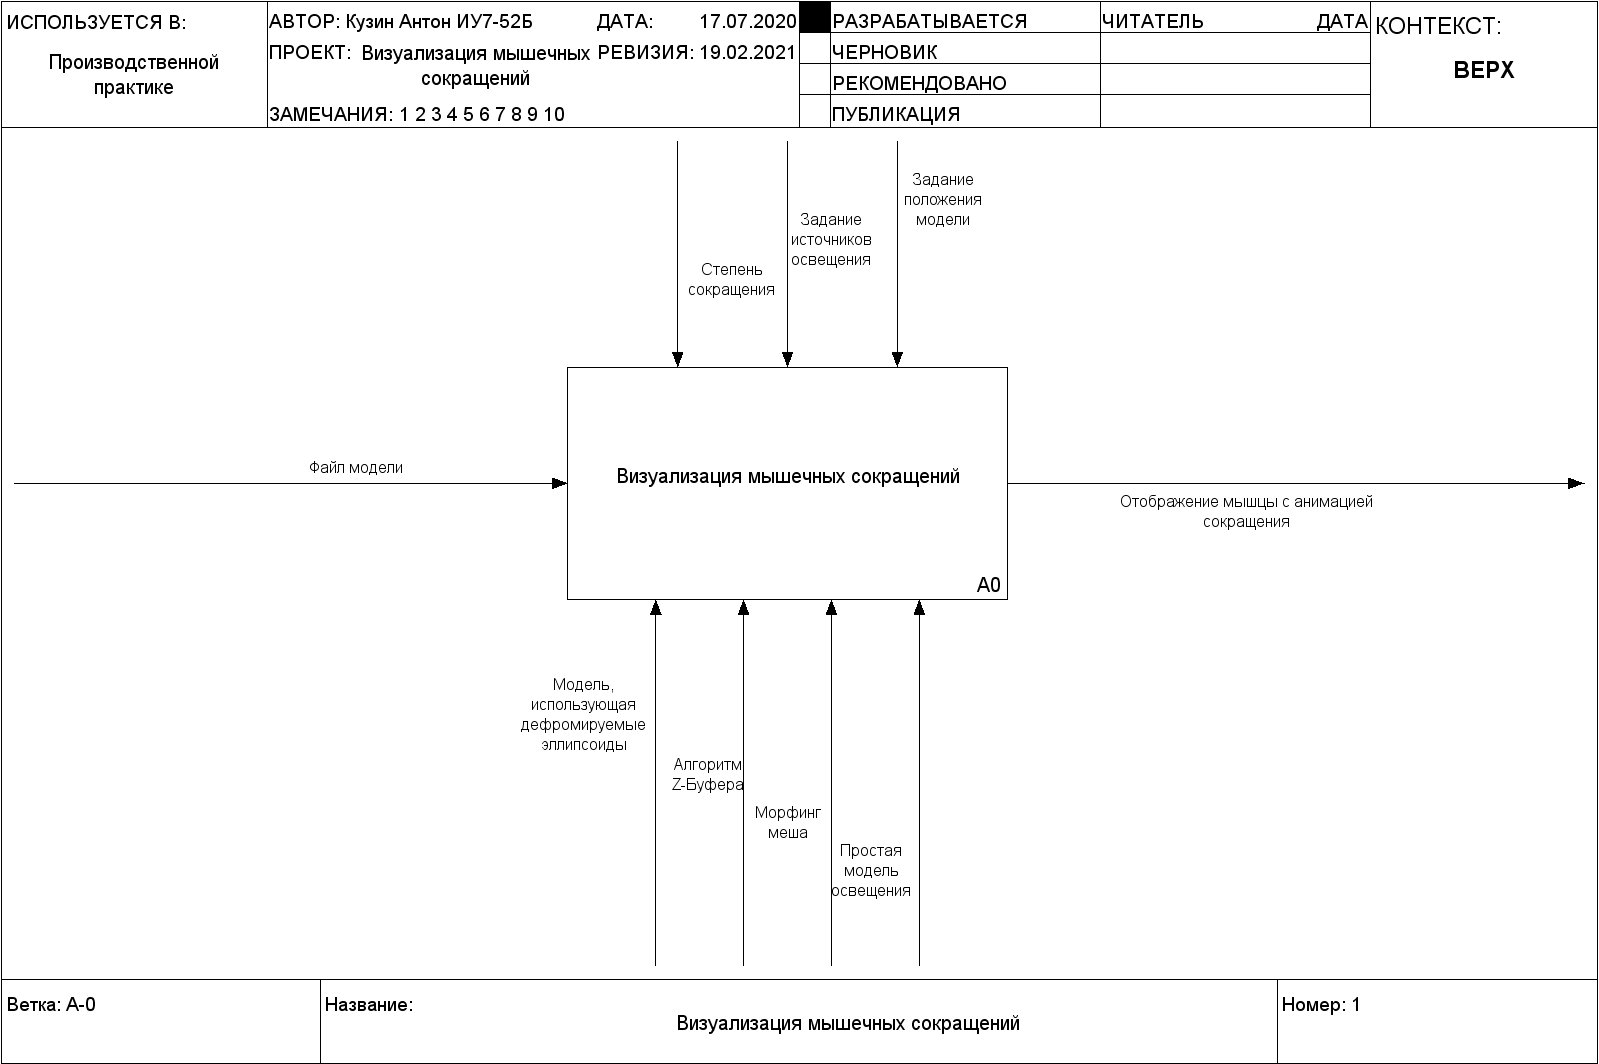
\includegraphics[height=0.5\paperheight, angle=90]{images/01_A-0}
	\caption[IDEF0 диаграмма, блок А0]{IDEF0 диаграмма, блок А0}
	\label{fig:01a-0}
\end{figure}
\begin{figure}[H]
	\centering
	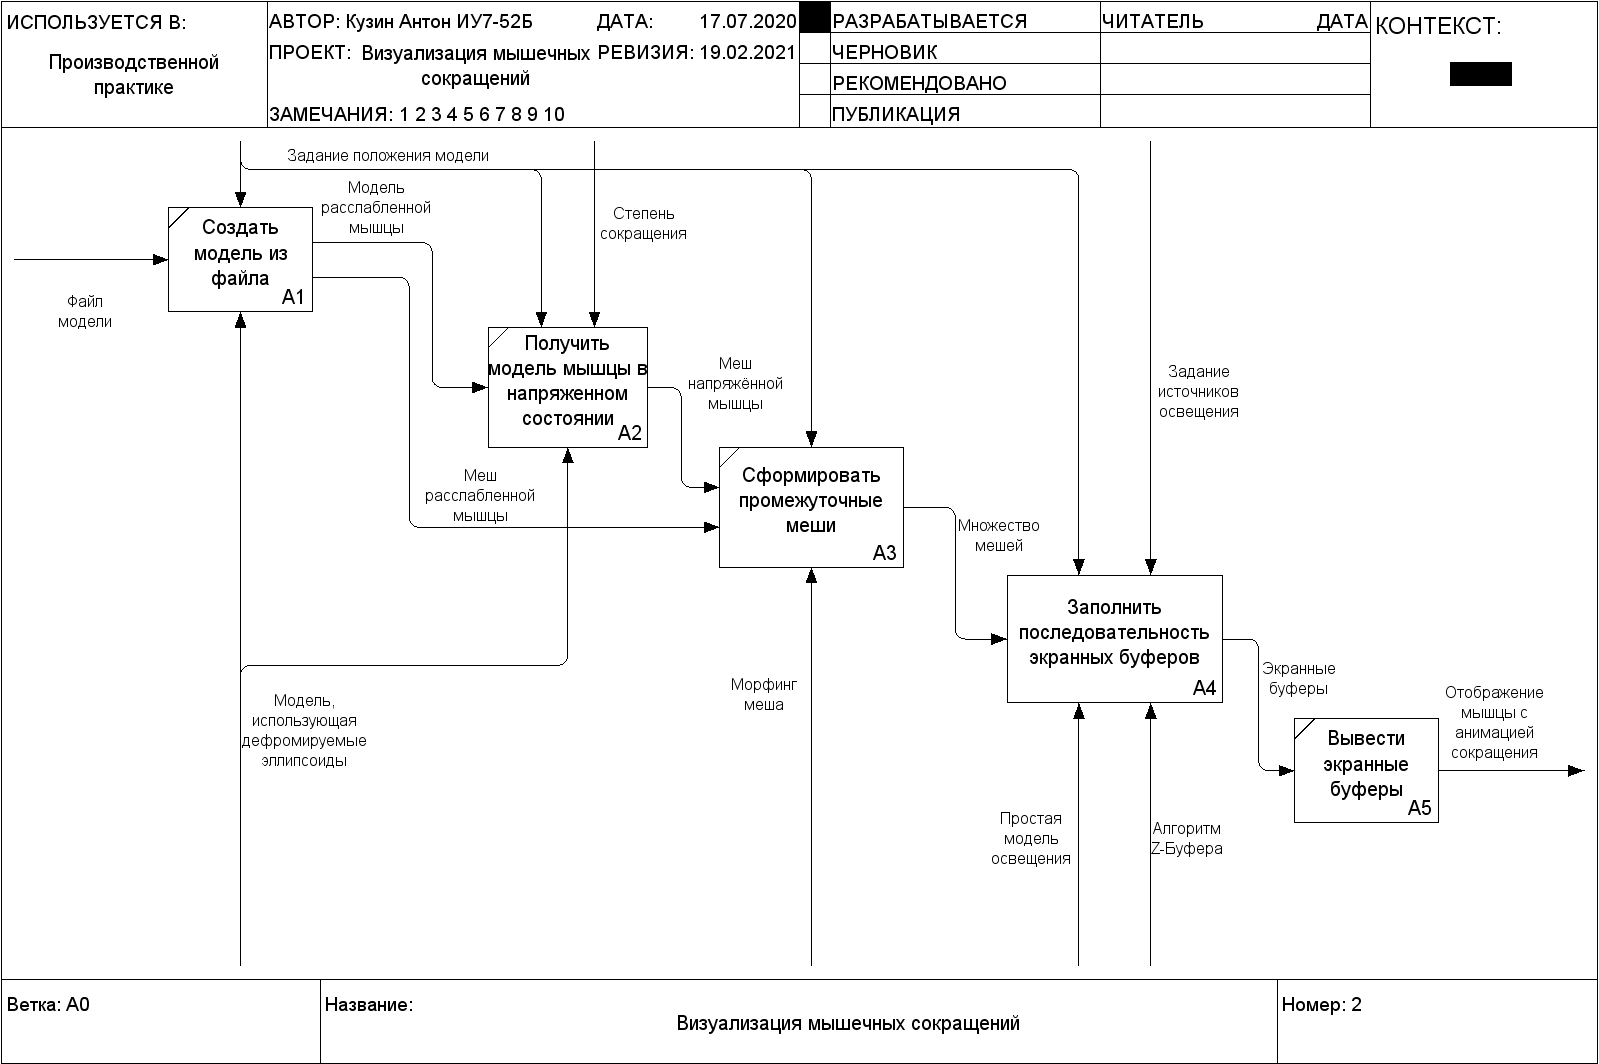
\includegraphics[height=0.5\paperheight, angle=90]{images/02_A0}
	\caption[Последовательность действий для отображения анимации сокращения мышцы]{Последовательность действий для отображения анимации сокращения мышцы}
	\label{fig:02a0}
\end{figure}

\section{Реализуемые алгоритмы алгоритмы}
\label{sec:algs}
\paragraph{Модель скелетных мышц}
В качестве модели аппроксимации скелетных мышц было решено использовать деформируемые эллипсоиды \cite{scheepers97}. Для представления сокращения параметры эллипсоида задаются с помощью математических уравнений, что позволяет сохранять объем и соотношение между высотой и шириной мышцы. Объем рассчитывается по формуле:
\begin{equation}
	v = \frac{4\pi abc}{3}
\end{equation}
Полагая $l'$ новой длиной мышцы, $r=\frac{a}{b}$, то 
\begin{equation}
	c'=\frac{l'}{2}
\end{equation}
\begin{equation}
	b'=\sqrt{\frac{3v}{4\pi rc'}}
\end{equation}
\begin{equation}
	a'=b'r
\end{equation}
Для визуализации изометрического сокращения мышцы соотношения r пересчитывается по формуле:
\begin{equation}
	r=(1-t+kt)r_n
\end{equation}
где $r_n$--соотношение $\frac{a}{b}$ в расслабленном состоянии, $t$--степень напряжённости $t\in [0,1]$, $k$--параметр контроля напряжения, который регулирует степень сжатия.

\par Поскольку в качестве метода моделирования полигональный, в связи с чем появляется необходимость в триангуляции эллипсоида. Алгоритм, представляющий эллипсоид, описанный его параметрами, можно описать следующими шагами:
\begin{enumerate}[1.]
	\item Построить куб в начале координат.
	\item Представить его в виде треугольных полигонов.
	\item Каждый полигон разбить на 4 других полигона.
	\item Нормализовать каждую вершину.
	\item К полученной сфере применить преобразования, умножив координаты точек на параметры эллипсоида.
\end{enumerate}
Шаг 3 можно выполнять рекурсивно произвольное количество раз, что приведёт к увеличению числа полигонов. Большая глубина рекурсии позволит сделать изображение более реалистичным, однако увеличит время необходимое на обработку изображения. В результате выполнения алгоритма мы получим эллипсоид, расположенный в начале координат.

\paragraph{Алгоритм z-буфера}
в общем виде может быть описан последовательностью таких шагов:
\begin{enumerate}[1.]
	\item Заполнить буфер кадра фоновым значением интенсивности или цвета.
	\item Заполнить z-буфер минимальным значением z.
	\item Преобразовать каждый многоугольник в растровую форму в произвольном порядке:
	\begin{enumerate}
		\item Для каждого пикселя в многоугольнике вычислить его глубину z.
		\item Сравнить глубину z со значением z в буфере в этой же позиции. Если z > Zбуфер, то записать атрибут этого пикселя в буфер кадра и заменить Zбуфер на z.
	\end{enumerate}
\end{enumerate}

\paragraph{Простая модель освещения} интенсивность рассчитывается по закону Ламберта c учётом рассеянного освещения, представленного константой:
\begin{equation}\label{lambert2}
I = I_{a}k_{a} + I_{l}k_{d}\cos \theta \qquad 0\leq\theta\leq\pi/2
\end{equation}
$I$ - интенсивность отражённого света, $I_{i}$ - интенсивность точечного источника, $k_{d}$ - коэффициент диффузного отражения ($0\leq k_{d}\leq 1$), $\theta$ - угол между направлением света и нормалью к поверхности, $I_{a}$ - интенсивность рассеянного света, $k_{a}$ - коэффициент диффузного отражения ($0\leq k_{a}\leq 1$).

\paragraph{Морфинг меша} можно разделить на два этапа: установление соответствия между полигонами начального и конечного состояний модели и интерполяция положения вершин. На рисунке \ref{fig:morphingalg} представлен алгоритм морфинга мешей, следует отметить что для установления связи между полигонами начала и конца не производится никаких вычислений, а каждому i-ому полигону начала в соответствие ставится i-ый полигон конца, это связано с тем, что объект источника и объект цели имеют одинаковую форму и одинаковое количество полигонов, в связи с чем предполагается, что для того, чтобы не нарушить целостность объекта необходимо сопоставить их в том же порядке.
\begin{figure}[H]
	\centering
	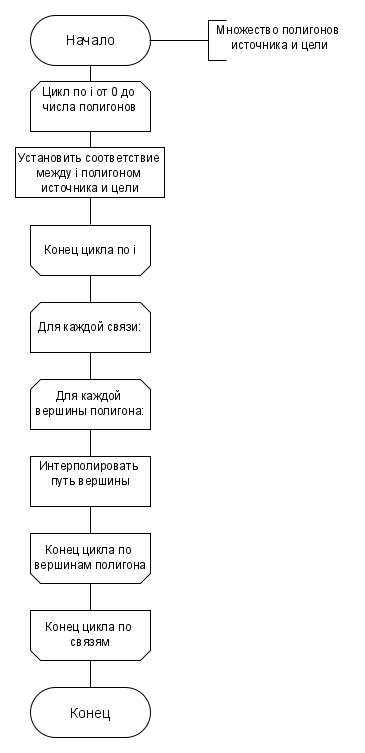
\includegraphics[width=0.7\linewidth]{images/morphing_alg}
	\caption[Алгоритм морфинга]{Алгоритм морфинга}
	\label{fig:morphingalg}
\end{figure}

\section{Вывод}
\label{sec:conc_constr}
В этом разделе были рассмотрены требования к программе, общий алгоритм ее работы, представлены схемы для реализации выбранных алгоритмов и математические формулы.
